\documentclass{pgnotes}

\title{EC2}

\begin{document}

\maketitle

Infrastructural services consist of compute, low-level storage and the networking required to connect them.
Compute is provided on AWS using a service called EC2.
Virtual Machines on EC2 are called Instances.

Instances are grouped into a virtual network called a VPC.
VPCs are important --- without them we wouldn't be able to connect to our virtual machines at all.

\section{Compute instances}
\label{sec:compute-instances}

The backbone IaaS compute service offered by AWS is Elastic Compute 2.
This allows you to create Virtual Machines on the AWS platform.
Many of their other services rely on EC2.
Other major cloud platforms (Azure, IBM, Google) all offer a basic virtual-machine compute service.
Virtual Machines created on AWS are known as EC2 instances (or just instances).

\subsection{EC2 instances}
\label{sec:ec2-instances}

To launch an instance, we must decide:

\begin{description}
\item[Instance Type]
  which sets the hardware configuration.
  Includes CPU family, numberof cores, clock speed, RAM.
\item[Operating System]
  template as available as an Amazon Machine Image (or AMI) that will be used to clone the image from.
\item[Storage:]
  The instance's virtual hard disk.
\item[VPC and Subnet]
  that the instance will be launched into.
\item[Security group]
  which defines what traffic is allowed in/out of individual EC2
  instances.
  Try to use shared/template ones rather than one per instance.
\end{description}

\subsection{Amazon Machine Image (AMI)}
\label{sec:amazon-machine-image-ami}

\begin{itemize}
\item
  On physical servers (and when dealing with on-site virtualisation
  systems) we often install an OS using an installer disk and work
  through the steps of the installer.
\item
  Cloud compute instances are normally created by cloning an image and
  running some minor post-installation tasks.
\item
  AWS uses the Amazon Machine Image (AMI) to clone a compute instance's
  virtual hard disk from.
\end{itemize}

\subsection{Amazon Linux}\label{amazon-linux}

There are a few different Linux distributions on AWS as AMIs, (as well as Windows).
One possible Linux flavour is Amazon Linux which is stripped-down for use as a cloud server and is maintained by AWS:

\begin{itemize}
\item
  By default, a user named \texttt{ec2-user} is provisioned. You can of
  course set up other users as you wish as on any OS.
\item
  It uses the RedHat \texttt{yum} package manager rather than
  \texttt{apt} as in Ubuntu / Debian. \emph{(You should be comfortable
  at this stage working with similar non-identical tools to broaden your
  experience and horizon!)}
\end{itemize}

\subsection{Remote Access}\label{remote-access}

Unlike some virtualisation solutions (e.g.~Xen server, Hyper-V), AWS provide no emulated Keyboard / Video / Mouse (KVM).
All operations must be carried out using remote access protocols like Secure Shell (SSH) or Remote Desktop Protocol.

\subsection{Key pairs}
\label{sec:key-pairs}

Some AMIs have a default username/password, but most including Amazon
Linux use a key-pair:

\begin{enumerate}
\item
  You generate a public / private key pair using \texttt{ssh-keygen}
\item
  You use the public key when creating EC2 instances.
\item
  Log in using \texttt{ssh} using your private key.
  Username for Amazon Linux is \texttt{ec2-user}.
\end{enumerate}


\section{Security groups}
\label{security-groups}

Security groups control a per-instance firewall that limits traffic into or out of each instance.
Each instance may have one or more security groups attached.

\subsection{Default security group}

Every instance created can have a default security group attached butthis leads to a few problems:

\begin{itemize}
\item
  Hard to get an overview of allowed/denied traffic to instances
  (security risk)
\item
  Hard to reconfigure allowed/denied traffic to a number of instances
  (time consuming, nuisance)
\end{itemize}

Instead it is preferable to create a security group and attach it as needed to instances in our VPC.

\subsection{Ingress rules}\label{sec:ingress-rules}

Ingress rules allow traffic in on a particular port (e.g. TCP 22 for SSH). 
We often use the IP range 0.0.0.0/0 as the source, meaning from anywhere on the internet.
We can lock this down to specific IP addresses or IP ranges (e.g.~your ISP). 

\subsection{Egress rules}\label{sec:egress-rules}

By default, security groups allow egress of all traffic from instances, so this doesn't need to be set up.

\section{Virtual private clouds}
\label{sec:virtual-private-clouds}

IaaS components (like EC2) are launched in Virtual Private Clouds (VPCs).

\subsection{Virtual Private Cloud (VPC)}

A VPC (Virtual Private Cloud)  is a virtual software-defined network to which your compute instances connect.
Essentially it's a software-defined multi-site data entre environment.
Each VPC \ldots{}

\begin{itemize}
\item
  \ldots{} is associated with a single specific region.
\item
  \ldots{} is owned by a single AWS account.
\item
  \ldots{} has a CIDR block of addresses, such as 10.0.0.0/16.
\end{itemize}

\subsubsection{IP addresses}

Classless Inter Domain Routing is a way to specify a range of IP addresses in a standard format.
An IPv4 address is a 32-bit identifier conventionally considered as 4 blocks of 8-bits, \autoref{fig:ipv4-address}

\begin{figure}[htbp]
  \centering
  
\includegraphics[width=0.5\linewidth]{ipv4_address}
  \caption{IPv4 address}
  \label{fig:ipv4-address}
\end{figure}

\subsubsection{CIDR blocks}

Common CIDR ranges are shown \autoref{fig:ip-address-classes}.

\begin{figure}[htbp]
  \centering
  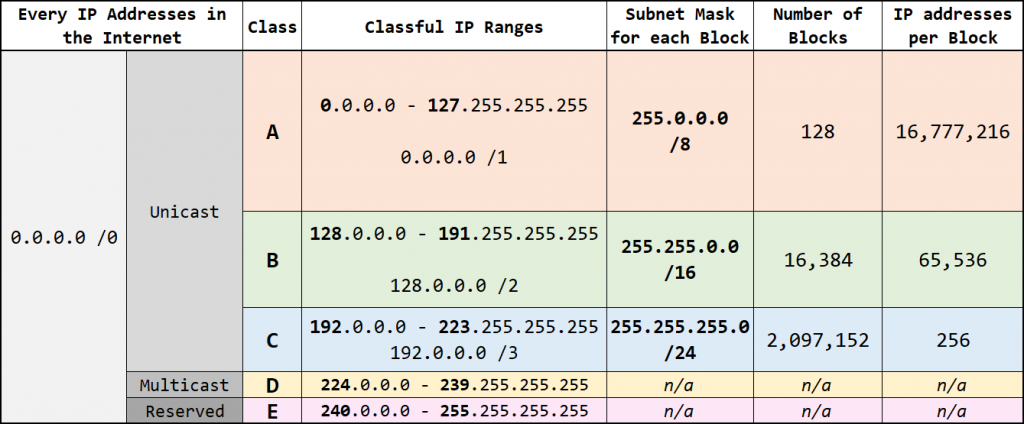
\includegraphics[width=1.0\linewidth]{ip_address_classes}
  \caption{Common CIDR ranges}
  \label{fig:ip-address-classes}
\end{figure}

\subsection{Subnets}

A VPC will normally contain one or more subnets. 
Each subnet:

\begin{itemize}
\item
  is associated with a single specific Availability Zone.
\item
  has a single CIDR-block of addresses, such as 10.0.1.0/24.
\item
  may contain one or more EC2 instances.
  Each EC2 instance therefore belongs to a particular VPC.
\end{itemize}

\subsection{Internet Gateway}

When a VPC (and its subnets) are created, it's actually isolated from the internet.
An Internet Gateway connects a VPC to the public internet.

There are some circumstances we'll see later on where we actually don't want a VPC to connect to the internet, but generally we do.
Therefore, except in some unusual configurations, every VPC will have an internet gateway attached to it.

\subsection{Route table(s)}

Route tables control how traffic is directed among the different subnets and into/out of the VPC.
They're not difficult to understand, but a misconfigured route table will generally cause problems.
Every VPC has a default route table that normally specifies that:
\begin{itemize}
\item Traffic for IP ranges within the VPC is local.
\item Traffic for IP ranges anywhere (0.0.0.0/0) must go through the internet gateway.
\end{itemize}


\section{Names and IDs}\label{names-and-ids}

Names are important to identify components.
We already know that AWS use text code names for the different regions and AZs.
As we create and use resources it's important to note the distinction between names we assign and Ids that are assigned by AWS:

\begin{description}
\item[Names]
  are assigned by you when creating components like VPCs, subnets, internet gateways, ec2 instances.
\item[Ids]
  are assigned by AWS when you create the same resources.
\end{description}

You can name things any way you like, but I tend to suggest you follow a pattern and avoid spaces!
\autoref{tab:iaas-naming} shows suggested suffix patterns I use (with the corresponding AWS prefixes for the ids)

\begin{table}[htbp]
  \centering
  \begin{tabular}{l l l}
    \toprule
    \textbf{Component type} & \textbf{Suggested name suffix} & \textbf{AWS name prefix}\\
    \midrule
    VPC & \texttt{\_VPC} & \texttt{vpc-}\\
    Subnet & \texttt{\_SN} & \texttt{sn-}\\
    Internet gateway & \texttt{\_IGW} & \texttt{igw-}\\
    Route table & \texttt{\_RTB} & \texttt{rtb-}\\
    \bottomrule
  \end{tabular}
  \caption{Naming suggestions and AWS Id prefixes}
  \label{tab:iaas-naming}
\end{table}


\end{document}

